\chapter{Diffusion des Lennard-Jones-Fluids}
Mit den im vorherigen Kapitel gefundenen Gitterkonstanten für die verschiedenen Agregatszustände, soll nun in diesem Kapitel das Diffusionsverhalten untersucht werden. 
\begin{compactitem}
 \item fest $\Leftrightarrow$ Gitterkonstante = $0.8$
 \item flüssig $\Leftrightarrow$ Gitterkonstante = $1.1$
 \item gasförmig $\Leftrightarrow$ Gitterkonstante = $1.4$
\end{compactitem}
Die grundsätzlichen Parameter bleiben unverändert.
\begin{figure}[h!]
	\centering
		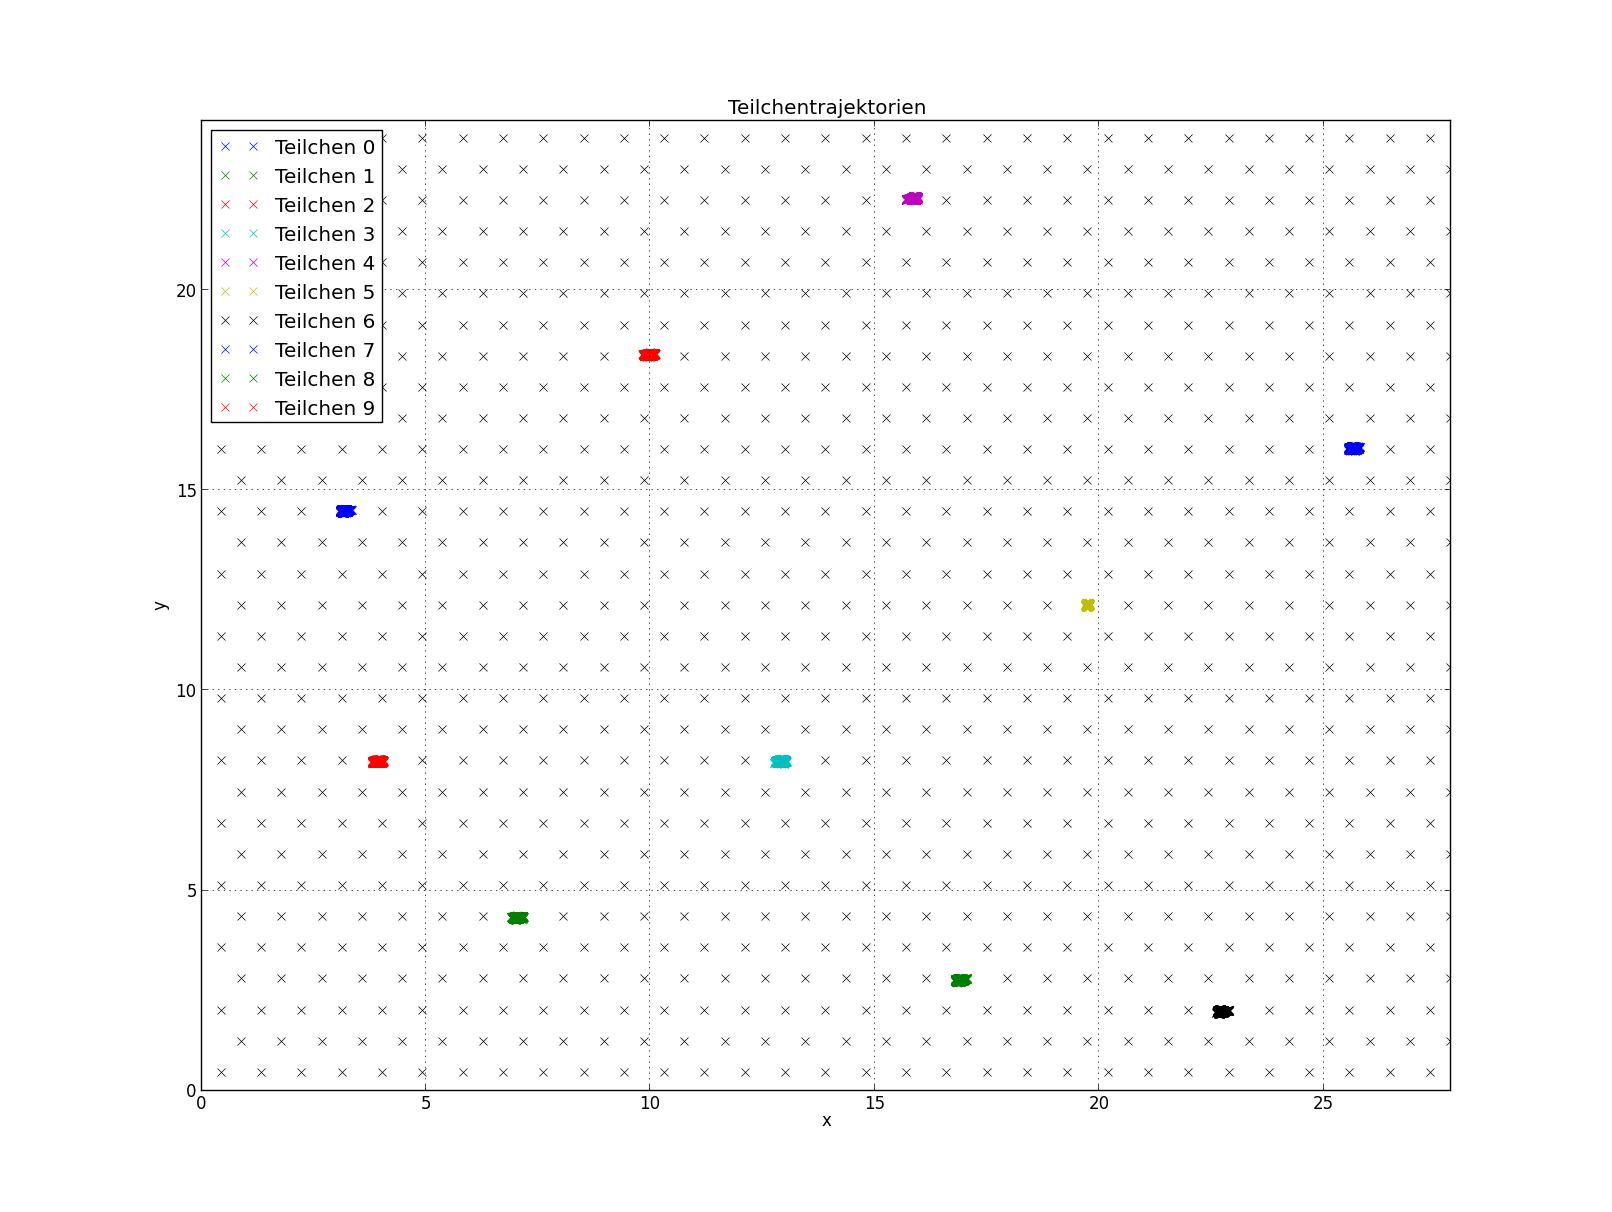
\includegraphics[width=0.70\textwidth]{img/Tra08.jpeg}
	\caption{Trajektorien von 10 zufällig gewählten Partikeln. Die Startpositionen aller Teilchen wurden in grau hinterlegt. Es zeigt sich, dass sich die Teilchen in einem festen Kristallgitter befinden. Da jedes Teilchen mit einer Startenergie (Geschwindigkeit) ausgestattet wurde, zeigen sich Zitterbewegungen um die Kristallposition. Diese Phase kann als fest bezeichnet werden.}
	\label{fig:Tra08}
\end{figure}
\begin{figure}[h!]
	\centering
		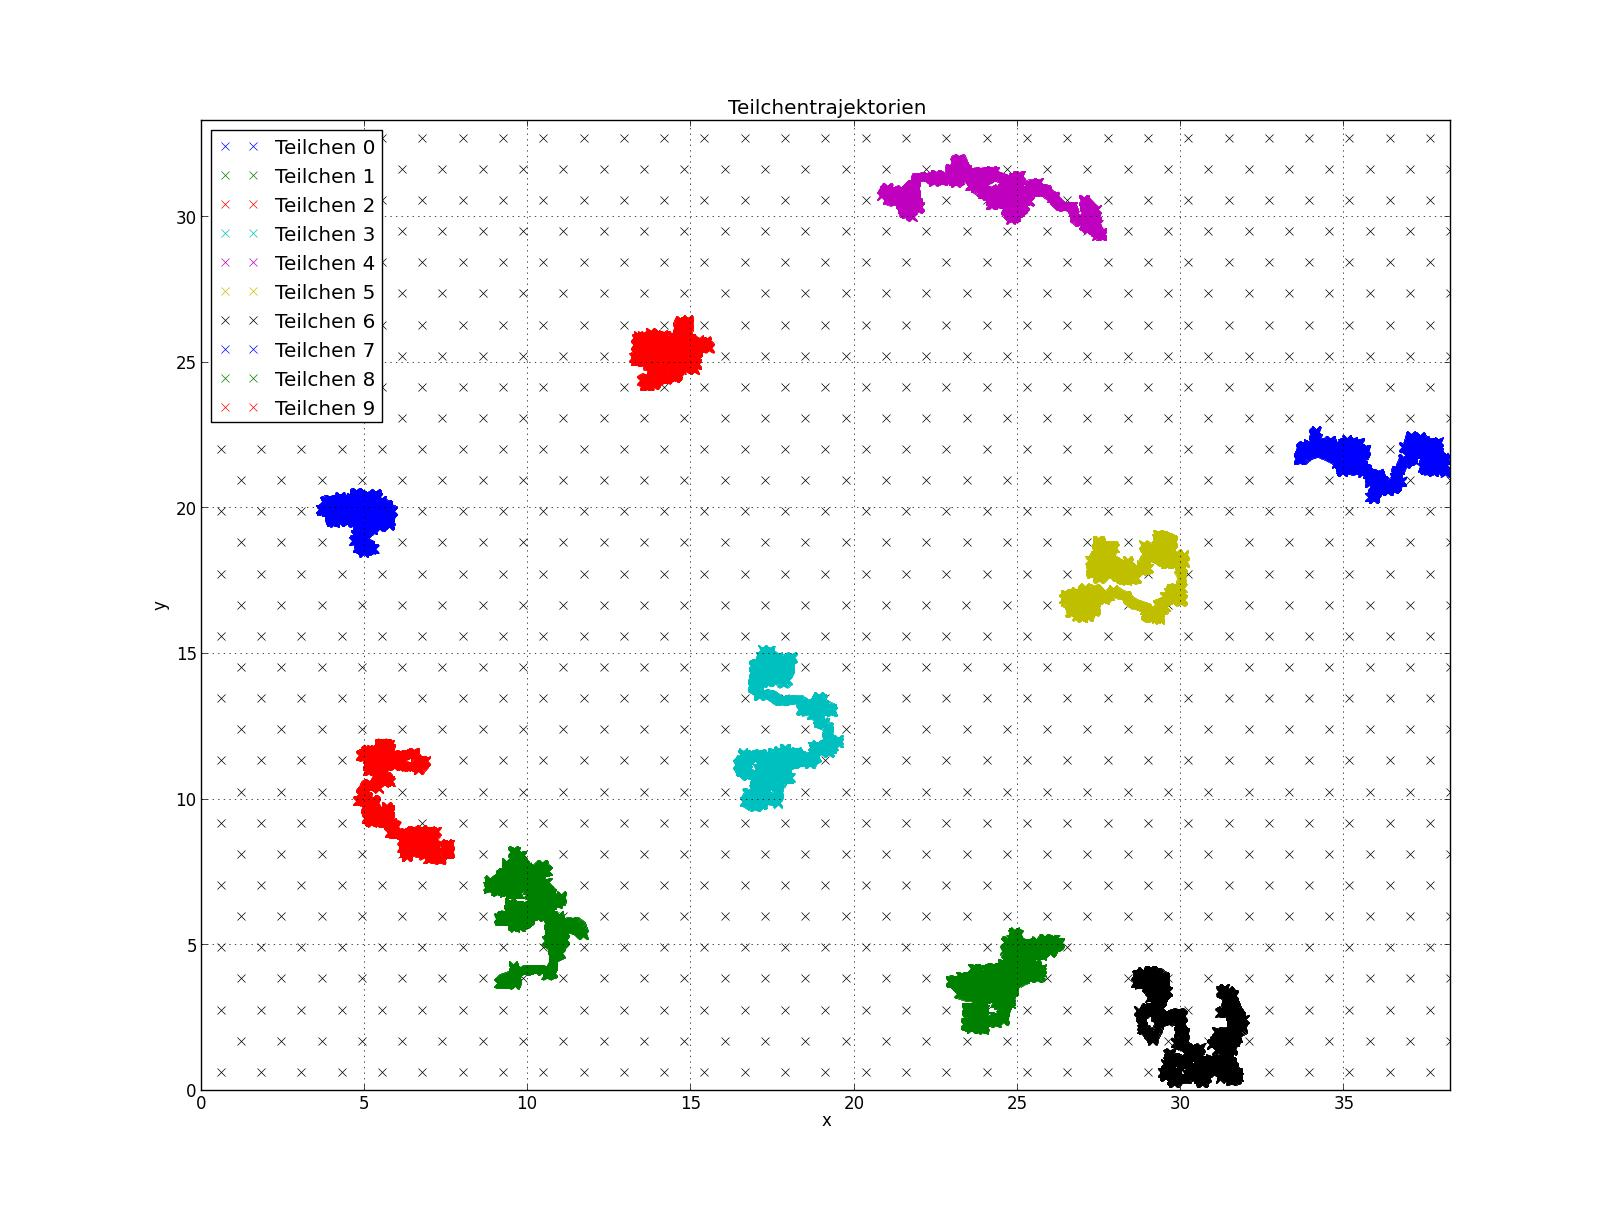
\includegraphics[width=0.70\textwidth]{img/Tra11.jpeg}
	\caption{Trajektorien von 10 zufällig gewählten Partikeln. Die Startpositionen aller Teilchen wurden in grau hinterlegt. Die Teilchen zeigen schwaches Diffusionsverhalten. Dieser Zustand wurde mit flüssig assoziiert.}
	\label{fig:Tra11}
\end{figure}
\begin{figure}[h!]
	\centering
		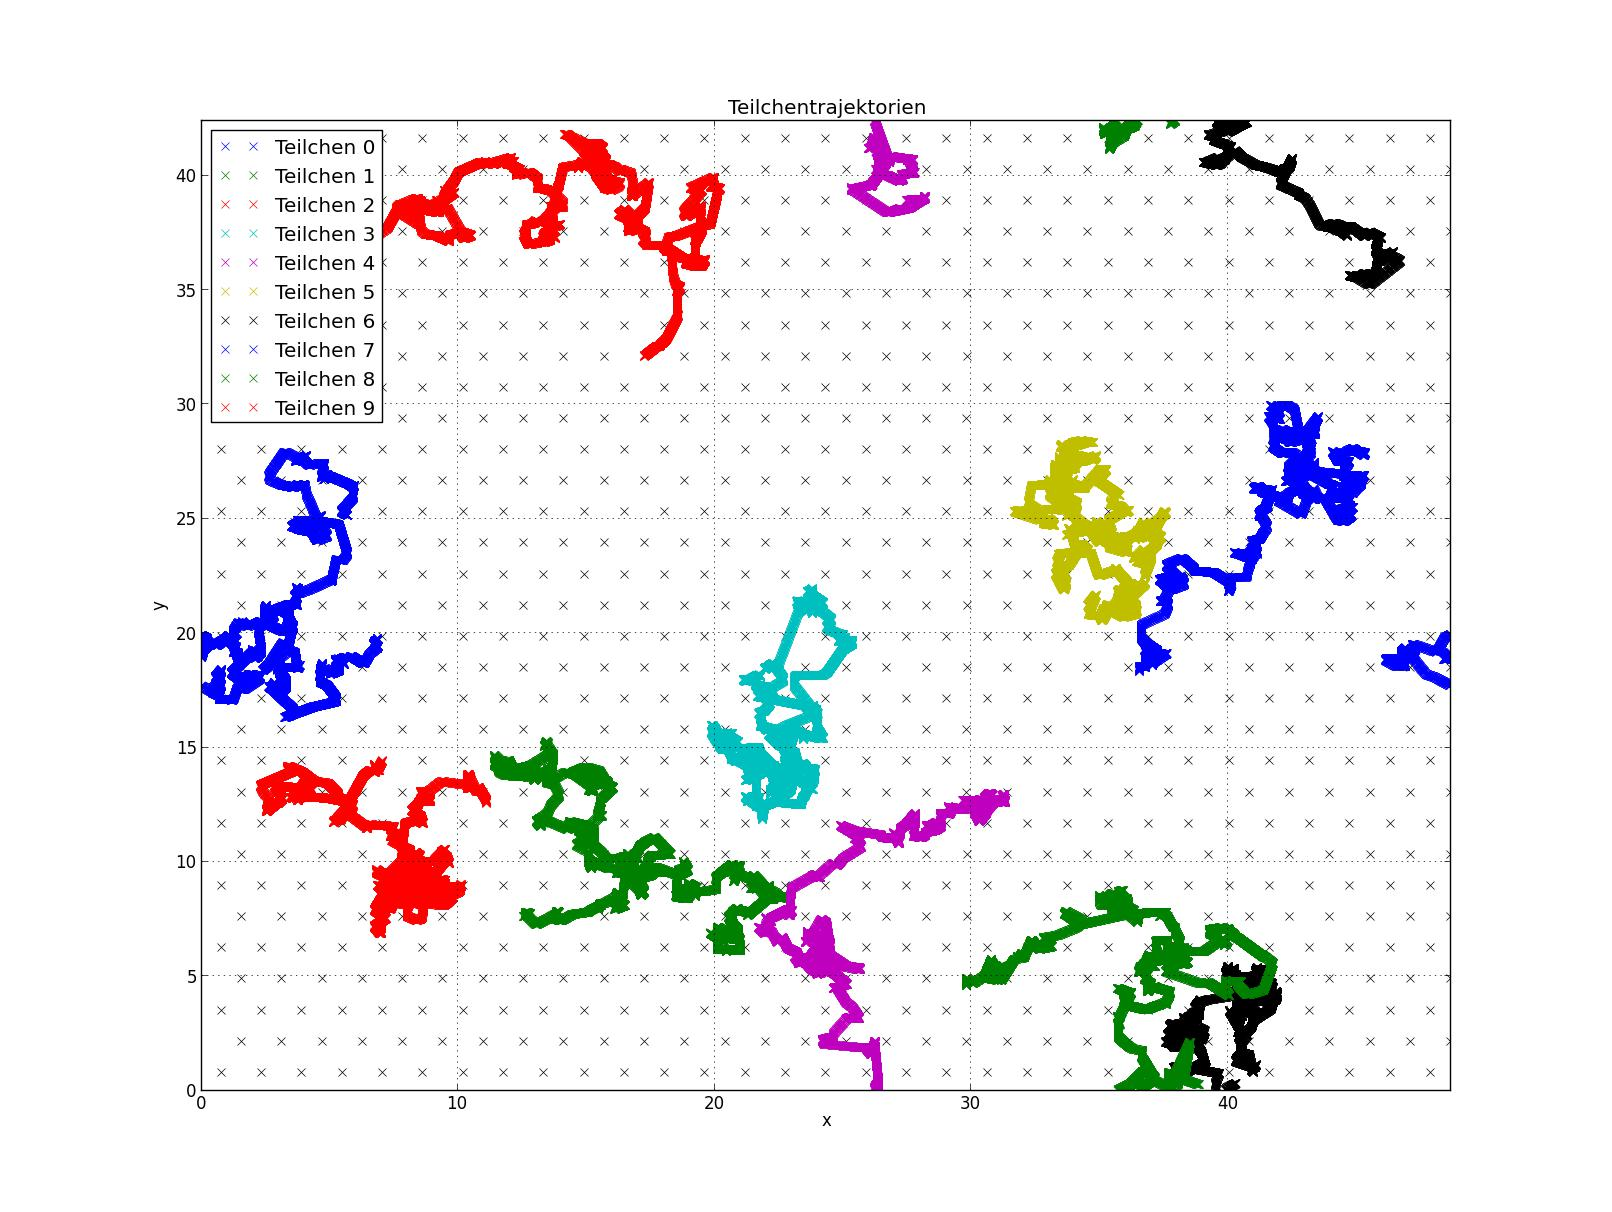
\includegraphics[width=0.70\textwidth]{img/Tra14.jpeg}
	\caption{Trajektorien von 10 zufällig gewählten Partikeln. Die Startpositionen aller Teilchen wurden in grau hinterlegt. Die Teilchen zeigen ausgeprägtes Diffusionsverhalten. Es kann von einem gasförmigen Zustand gesprochen werden.}
	\label{fig:Tra14}
\end{figure}